Here we will explain how we developed our AXI interconnect, first explaining how it works as a stand-alone component, and then how we inserted it into the Processor.


{\color{Blue}{\subsection{Block Design}}}
In the figure \ref{HLBD} is reported the Block Diagram of the AXI interconnect we developed.

\begin{figure}[h]
  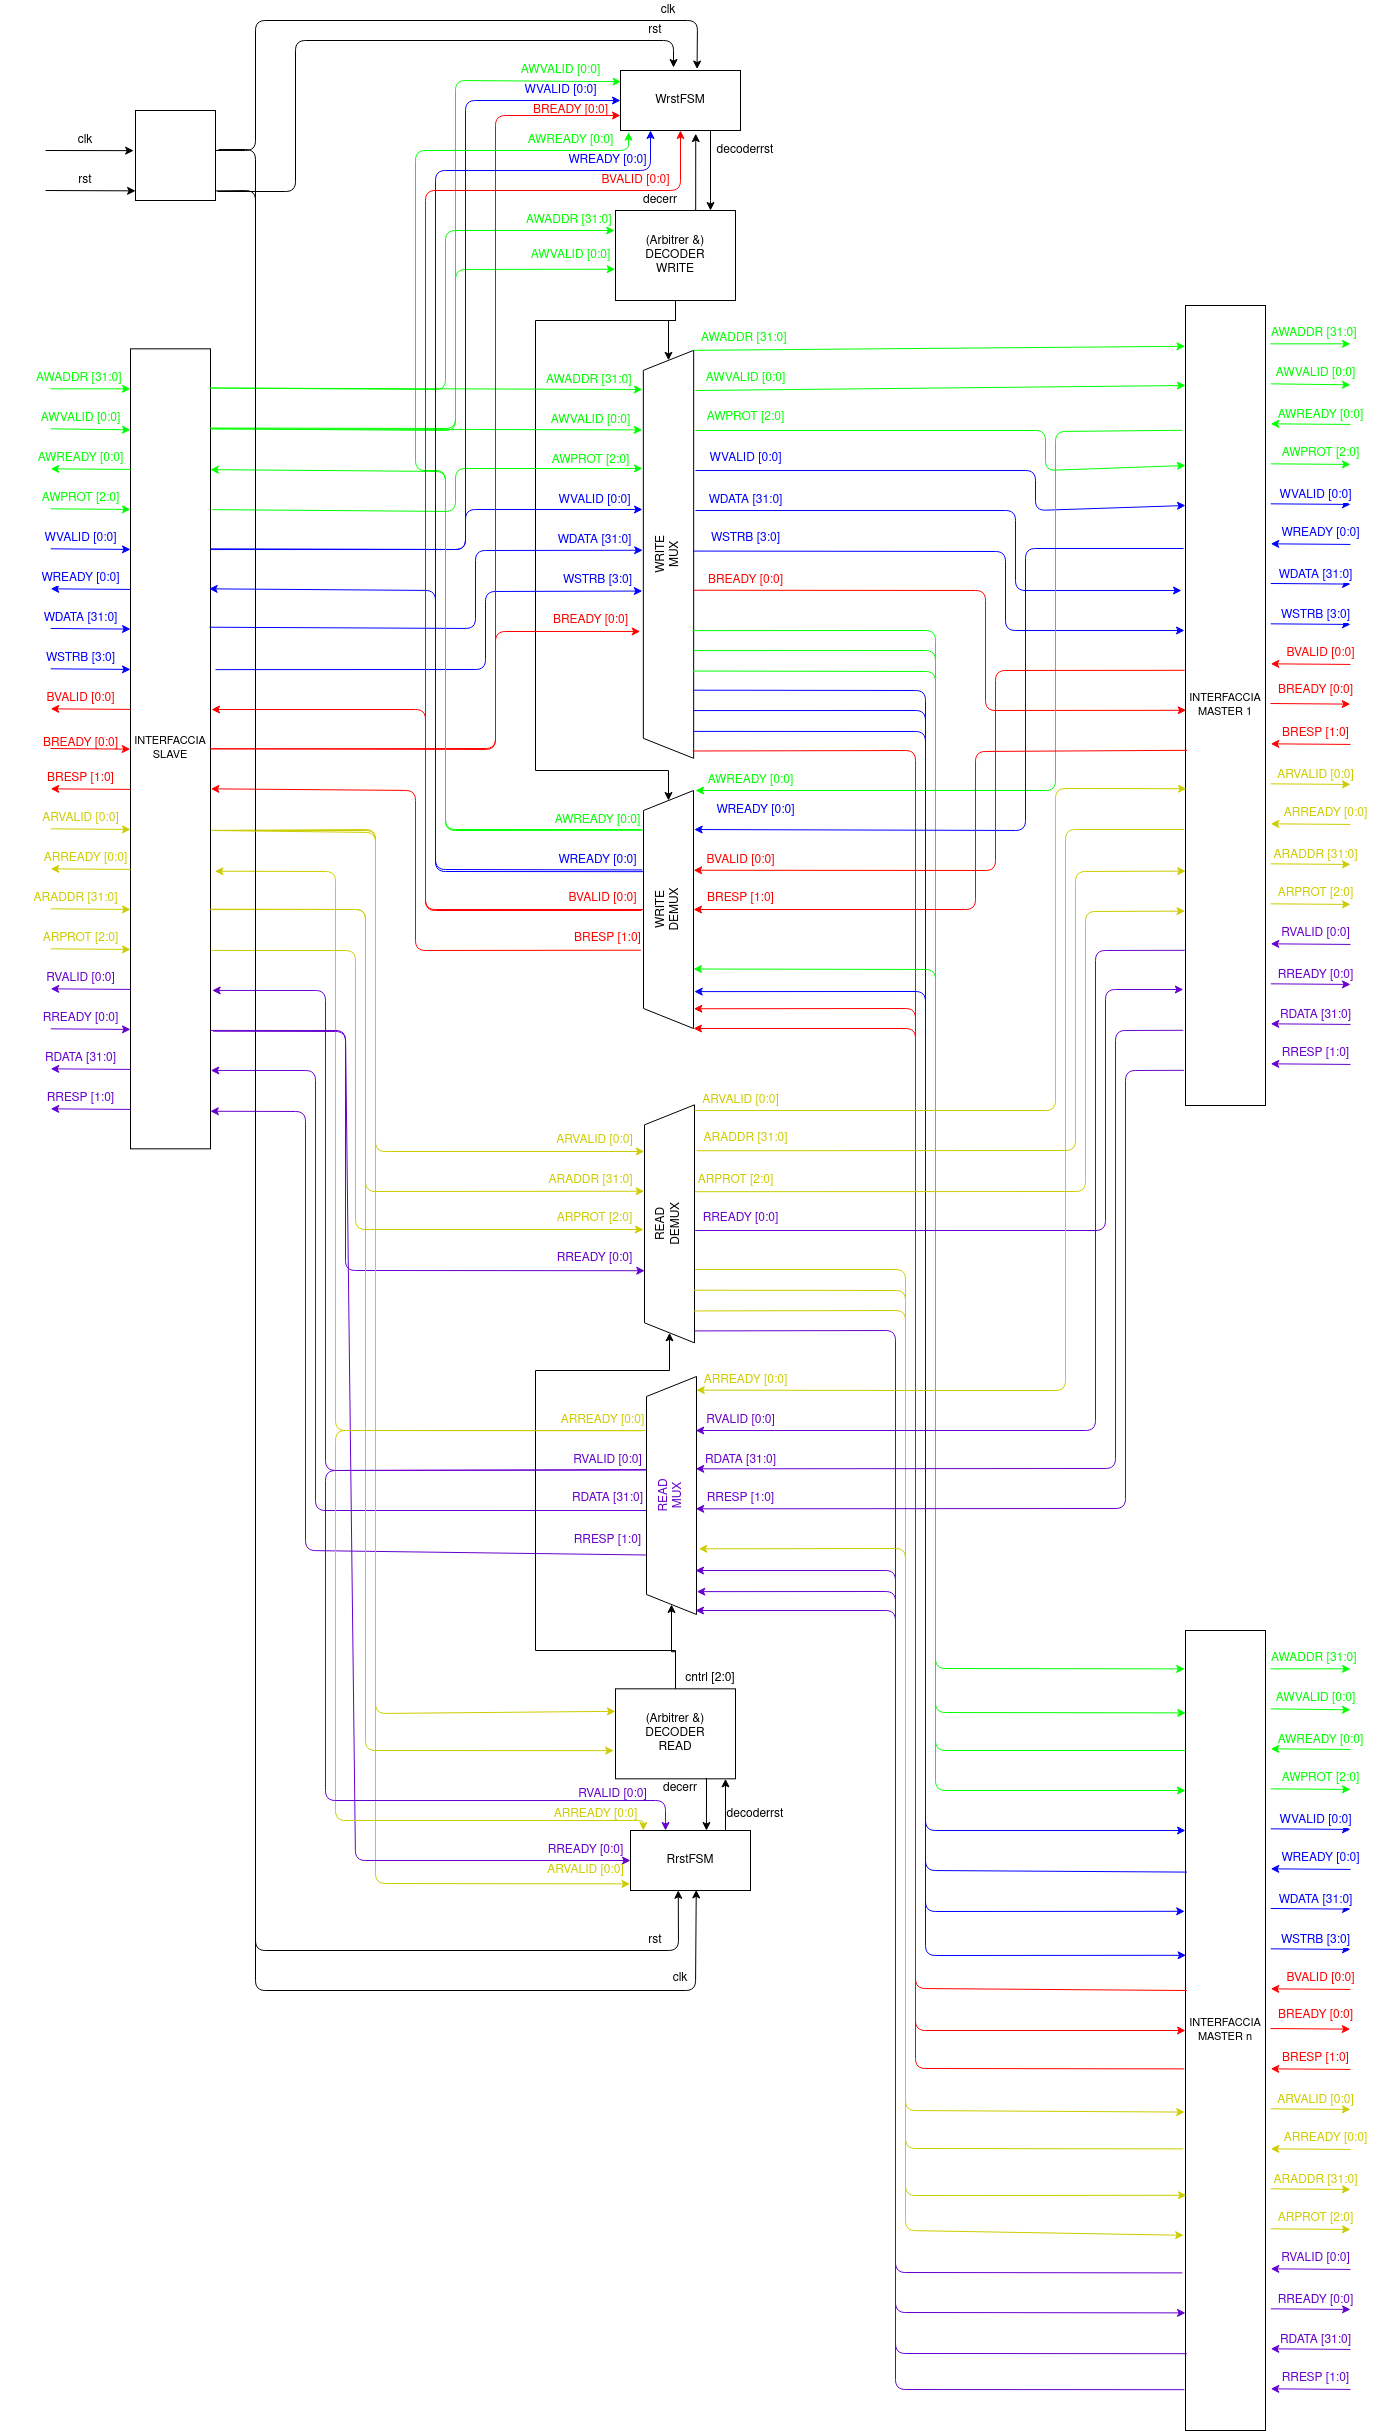
\includegraphics[width=0.9\textwidth, angle=0]{"./../../img/Images/highLevel.png"}
  \caption{highLevel block diagram}
  \label{HLBD}
\end{figure}

{\color{Blue}{\subsection{Coupling}}}
The coupling is achieved by the Muxers and Demuxers, driven by the Decoders which reads the Address and couple the address to the correspective slave.

{\color{Blue}{\subsection{Handshake}}}
The handshake's signals are checked by the FSM that will drive the Decoders to signal when the address is valid and when it's not.

{\color{Blue}{\subsection{Errors}}}
There are 2 types of error:
The ones raised by the slave (and are generated by slave and so pass through the AXI interconnect)
The ones raised if the address isn't mapped; in such a case we have an ad-hoc fake slave that sends the error to the master.

{\color{Blue}{\subsection{Integration inside the processor}}}
We managed to put our AXI right inside the processor without any fake component.
